
\chapter[Bài tập: Độ lệch pha giữa các đại lượng trong mạch điện xoay chiều]{Bài tập: Độ lệch pha giữa các đại lượng\\ trong mạch điện xoay chiều}
\section{Lý thuyết}
\subsection{Xác định độ lệch pha giữa các đại lượng trong mạch điện}
\subsubsection{Độ lệch pha giữa dòng điện và điện áp}

\begin{tabular}{|m{8em}|m{8em}|m{18em}|}
	\hline
	\multicolumn{2}{|l|}{\thead{Cấu tạo đoạn mạch}}                                                 & \thead{Độ lệch pha giữa $u$ và $i$}                           \\ \hline
	{\begin{tabular}[c]{@{}l@{}}\textbf{Mạch điện chứa}\\ \textbf{một phần tử}\end{tabular}} & \textbf{Mạch chứa $R$} & $$\varphi = \varphi_u-\varphi_i = 0$$                            \\ \cline{2-3} 
	& \textbf{Mạch chứa $L$} & $$\varphi = \varphi_u-\varphi_i = \dfrac{\pi}{2}\ \text{rad} $$  \\ \cline{2-3} 
	& \textbf{Mạch chứa $C$} & $$\varphi = \varphi_u-\varphi_i = -\dfrac{\pi}{2}\ \text{rad} $$ \\ \hline
	\multicolumn{2}{|l|}{\textbf{Mạch $R$, $L$, $C$ nối tiếp}}                                                & $$\tan \varphi = \dfrac{Z_L-Z_C}{R}$$                            \\ \hline
\end{tabular}
\subsubsection{Giản đồ vectơ trượt trong các bài toán về pha}
Nguyên tắc vẽ: tuân theo nguyên tắc cộng điện áp
\begin{equation*}
	u = u_R + u_L + u_C
\end{equation*}
\begin{center}
	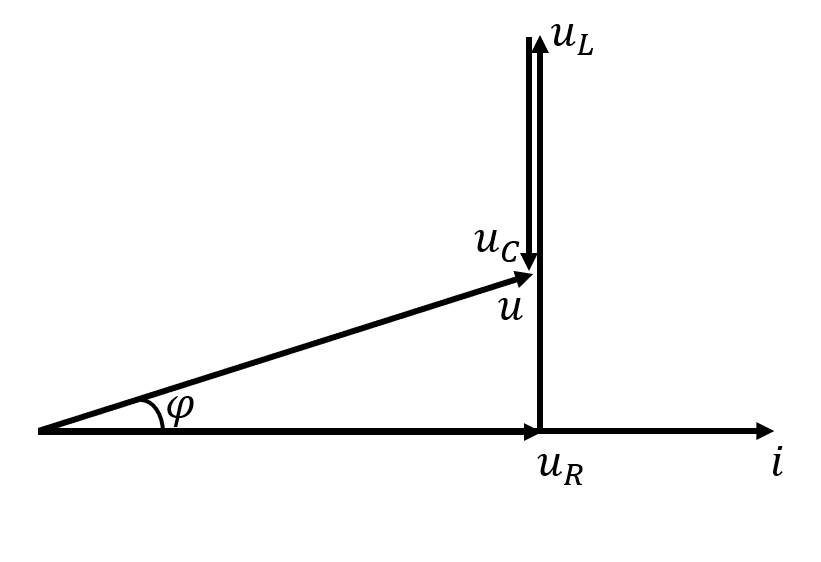
\includegraphics[scale=0.4]{../figs/VN12-PH-19-A-011-4-V2-1.png}
\end{center}



\subsection{Xác định phần tử của mạch điện (bài toán hộp đen)}
Xét mối liên hệ về pha của dòng điện ($\varphi_i$) và điện áp ($\varphi_u$), ta có các trường hợp sau:
\begin{center}
	\begin{tabular}{|m{10em}|m{9em}|m{9em}|m{9em}|}
		\hline
		&\thead{$u$ chậm pha hơn $i$} & \thead{$u$ cùng pha với $i$} & \thead{$u$ nhanh pha hơn $i$} \\
		\hline
		\textbf{Mạch điện chứa một phần tử} & Mạch chứa $C$ & Mạch chứa $R$ & Mạch chứa $L$ \\
		\hline
		{\begin{tabular}[c]{@{}l@{}}\textbf{Mạch điện chứa hai}\\ \textbf{phần tử khác loại}\end{tabular}} & Mạch chứa $R$, $C$ & & Mạch chứa $R$, $L$ \\
		\cline{2-4}
		&Mạch chứa $L$, $C$ với $Z_L < Z_C$& Mạch chứa $L$, $C$ với $Z_L = Z_C$&Mạch chứa $L$, $C$ với $Z_L > Z_C$ \\
		\hline
		\textbf{Mạch $R$, $L$, $C$ nối tiếp} & Mạch có tính dung kháng: $Z_L <Z_C$& Mạch có cộng hưởng điện: $Z_L =Z_C$ & Mạch có tính cảm kháng: $Z_L >Z_C$\\
		\hline
	\end{tabular}
\end{center}
\luuy{\begin{center}\textbf{Trường hợp cuộn dây không thuần cảm}\end{center}
	
	Xem cuộn dây không thuần cảm như hai phần tử $r$, $L$ mắc nối tiếp.}


\section{Mục tiêu bài học - Ví dụ minh họa}
\begin{dang}{Dựa vào phương trình dòng điện, điện áp, suất điện động  và giản đồ Fresnel để xác định độ lệch pha giữa các đại lượng\\ trong mạch điện xoay chiều}
	\viduii{2}{Một đoạn mạch gồm tụ điện mắc nối tiếp với một cuộn dây. Điện áp giữa hai đầu cuộn dây lệch pha $\dfrac{\pi}{3}$ so với cường độ dòng điện và lệch pha $\dfrac{\pi}{2}$ so với điện áp hai đầu đoạn mạch. Biết điện áp hiệu dụng giữa hai đầu đoạn mạch bằng $\SI{100}{\volt}$, khi đó điện áp hiệu dụng trên tụ điện và cuộn dây lần lượt là
		\begin{mcq}(2)
			\item $\SI{60}{\volt}$ và $60\sqrt 3 \ \text V$.
			\item $200\ \text V$ và $100 \sqrt 3 \ \text V$.
			\item $60\sqrt 3 \ \text V$ và $100\ \text V$.
			\item $100 \sqrt 3 \ \text V$ và $200\ \text V$.
	\end{mcq}}
	{\begin{center}
			\textbf{Hướng dẫn giải}
		\end{center}
		Biểu diễn các vectơ điện áp lên giản đồ vectơ trượt:
		\begin{center}
			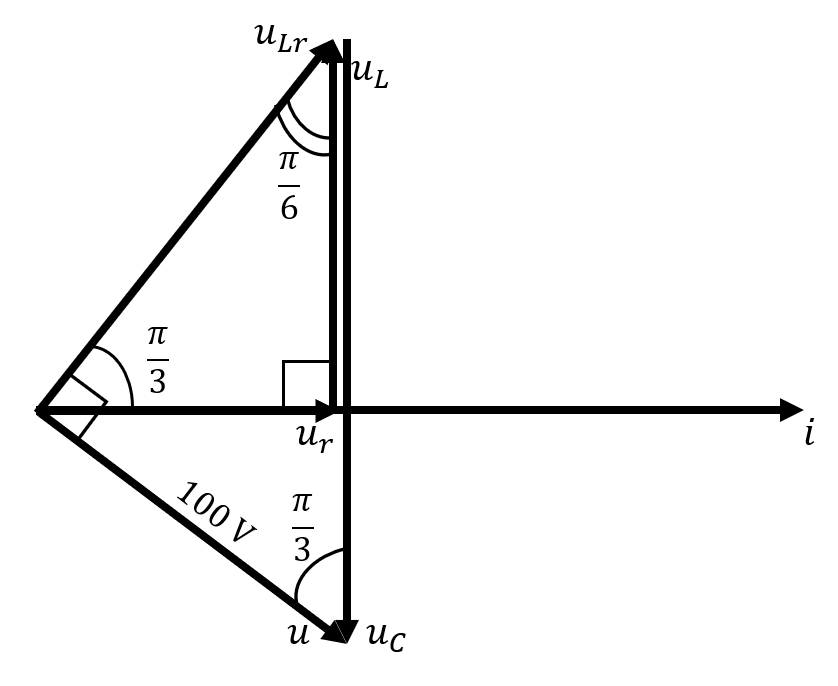
\includegraphics[scale=0.4]{../figs/VN12-PH-19-A-011-4-V2-2.png}
		\end{center}
		
		Áp dụng định lí hàm số sin:
		\begin{equation*}
			\dfrac{100}{\sin \dfrac{\pi}{6}} = \dfrac{u_{Lr}}{\sin\dfrac{\pi}{3}} = \dfrac{u_{C}}{\sin \dfrac{\pi}{2}},
		\end{equation*}
		ta được
		\begin{equation*}
			\dfrac{100}{\sin \dfrac{\pi}{6}} = \dfrac{u_{Lr}}{\sin\dfrac{\pi}{3}} \Rightarrow u_{Lr} = 100\sqrt 3\ \text V,
		\end{equation*}
		và 
		\begin{equation*}
			\dfrac{100}{\sin \dfrac{\pi}{6}} = \dfrac{u_{C}}{\sin \dfrac{\pi}{2}} \Rightarrow u_{C} = 200\ \text V.
		\end{equation*}
		
		\textbf{Đáp án: B.}
	}
	
	\viduii{3}{Đặt điện áp $u =100 \sqrt 6 \cos \left(100\pi t -\dfrac{\pi}{3}\right)\ \text{V}$ vào hai đầu đoạn mạch $RLC$ ghép nối tiếp theo đúng thứ tự thì $U_{RL} =\dfrac{U_C}{2} = 100\ \text{V}$. Viết biểu thức $u_{RL}$.
		\begin{mcq}
			\item $u_{RL} = 100\sqrt 2 \cos \left (100\pi t + \dfrac{\pi}{6}\right)\ \text{V}.$
			\item $u_{RL} = 100 \cos \left (100\pi t - \dfrac{\pi}{6}\right)\ \text{V}.$
			\item $u_{RL} = 100\sqrt 2 \cos \left (100\pi t - \dfrac{\pi}{6}\right)\ \text{V}.$
			\item $u_{RL} = 100 \cos \left (100\pi t + \dfrac{\pi}{6}\right)\ \text{V}.$
		\end{mcq}
	}
	{
		\begin{center}
			\textbf{Hướng dẫn giải}
		\end{center}
		Điện áp giữa hai đầu tụ điện $C$:
		$$U_{RL} =\dfrac{U_C}{2} = 100\ \text{V} \Rightarrow U_C = 200\ \text{V}.$$
		
		Điện áp hiệu dụng giữa hai đầu mạch chính:
		$$U=\dfrac{U_0}{\sqrt 2} = 100\sqrt 3\ \text{V}.$$
		
		Độ lệch pha: $\varphi_u = -\dfrac{\pi}{3}$.
		
		Ta thấy: $U_C^2 =U^2 +U^2_{RL}$ nên $\vec U$ vuông góc với $\vec U _{RL}$.
		
		Ta có giản đồ Fresnel:
		\begin{center}
			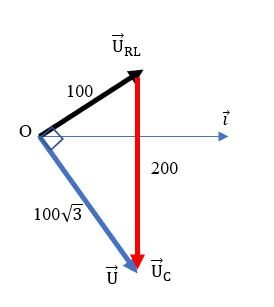
\includegraphics[scale=0.9]{../figs/VN12-PH-19-A-011-4-V2-4.JPG}
		\end{center}
		
		Với $U_{0RL} =U_{RL} \sqrt 2 =100 \sqrt 2\ \text{V}$; $u_{RL}$ nhanh pha $\dfrac{\pi}{2}$ so với $u$.
		
		Suy ra: $$\varphi_{u_{RL}} =\varphi_U + \dfrac{\pi}{2} = \dfrac{\pi}{6}.$$
		
		Biểu thức $u_{RL}$:
		$$u_{RL} = 100\sqrt 2 \cos \left (100\pi t + \dfrac{\pi}{6}\right)\ \text{V}.$$
		
		\textbf{Đáp án: A.}
	}
	
	
\end{dang}
\begin{dang}{Xác định phần tử mạch điện chưa biết trong bài toán hộp đen}
	\viduii{2}{Cho mạch điện xoay chiều gồm một tụ điện mắc nối tiếp với đoạn mạch X. Để dòng điện trong mạch chậm pha hơn điện áp một góc $\dfrac{\pi}{3}\ \text{rad}$ thì đoạn mạch X gồm những phần tử nào?
		\begin{mcq}(4)
			\item $L$.
			\item $R$, $L$.
			\item $R$.
			\item $R$, $C$.
		\end{mcq}
	}
	{\begin{center}
			\textbf{Hướng dẫn giải}
		\end{center}
		Để dòng điện trong mạch chậm pha hơn điện áp một góc $\dfrac{\pi}{3}\ \text{rad}$ thì ta có các trường hợp:
		\begin{itemize}
			\item Mạch chỉ chứa $L$ (loại vì không có $C$);
			\item Mạch chứa $R$, $L$ mắc nối tiếp (loại vì không có $C$);
			\item Mạch chứa $R$, $L$, $C$ mắc nối tiếp với $Z_L >Z_C$.
		\end{itemize}
		
		Vì mạch điện đã có sẵn tụ điện mắc nối tiếp với đoạn mạch X, nên đoạn mạch $X$ chứa hai phần tử là $R$ và $L$.
		
		\textbf{Đáp án: B.}
	}
	\viduii{3}{ Cho mạch điện xoay chiều như hình vẽ 
		\begin{center}
			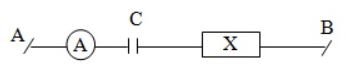
\includegraphics[scale=0.7]{../figs/VN12-PH-19-A-011-4-V2-3.JPG}
		\end{center}
		X là hộp đen chứa 1 phần tử: $R$ hoặc $L$ hoặc $L,r$ hoặc $C$, biết $u_\text{AB} = 100\sqrt 2 \cos 100 \pi t\ \text{V}$; $I_A = \sqrt 2\ \text{A}$; $P=100\ \text{W}$, $C = \dfrac{10^{-3} }{3\pi}\ \text{F}$, $i$ trễ pha hơn $u_\text{AB}$. Tìm cấu tạo X và giá trị của phần tử.
		\begin{mcq}
			\item Cuộn dây thuần cảm $L=\dfrac{4}{5\pi}\ \text{H}$.
			\item Cuộn dậy không thuần cảm $r =50\ \Omega, L =\dfrac{4}{5\pi}\ \text{H}$.
			\item Điện trở thuần $R =50\ \Omega$.
			\item Tụ điện $C = \dfrac{10^{-4}}{\pi}\ \text{F}$.
		\end{mcq}
	}
	{\begin{center}
			\textbf{Hướng dẫn giải}
		\end{center}
		Theo giả thiết $i$ trễ pha hơn $u_\text{AB}$ và mạch tiêu thụ điện suy ra: hộp đen là một cuộn dây có $r \neq  0$.
		
		Ta có:
		$$P = I^2r \Rightarrow r = \dfrac{P}{I^2} = 50\ \Omega.$$
		
		Mặc khác: 
		$$r^2 + (Z_L - Z_C)^2 = \dfrac{U^2_{\text{AB}}}{I^2
		} \Rightarrow |Z_L - Z_C| = \sqrt {\dfrac{U^2_{\text{AB}}}{I^2} -r^2} = \sqrt {\dfrac{100^2}{(\sqrt 2)^2} -50^2}.$$
		
		Thay $Z_C =\dfrac{1}{C\omega} = 30 \ \Omega$ suy ra $Z_L = 80\ \Omega$.
		
		Vậy độ tự cảm của cuộn cảm là
		$$L =\dfrac{Z_L}{\omega} = \dfrac{4}{5\pi} \ \text{H}.$$
		
		\textbf{Đáp án: B.}}
\end{dang}